\documentclass{article}

\usepackage[utf8]{inputenc}
\usepackage[backend=biber, style=apa]{biblatex}
\addbibresource{references.bib}

\usepackage{amsmath}     % For advanced math environments and symbols
\usepackage{amssymb}     % For mathematical symbols
\usepackage{amsthm}      % For theorem, lemma, proof environments
\usepackage{listings}
\usepackage{xcolor}
\usepackage{listings}    % For including actual code snippets
\usepackage{geometry}    % For setting page margins
\usepackage{hyperref}    % For clickable links and better PDF structure
\usepackage{graphicx}    % For including diagrams/images
\usepackage{tikz}

\usetikzlibrary{graphs, arrows.meta, positioning}

\tikzset{
task/.style={
    rectangle, 
    draw=blue!70, 
    fill=blue!10, 
    rounded corners, 
    minimum size=8mm, 
    font=\small\bfseries
}}

% --- Document Settings ---
\geometry{
    a4paper,
    margin=1in,
}
\hypersetup{
    colorlinks=true,
    linkcolor=blue,
    filecolor=blue,
    urlcolor=blue,
}

\title{A discussion on \emph{Optimal Scheduling of 2-Processor Systems}}
\author{Caleb Burke / 658780838}
\date{\today}

% --- Custom commands ---
\newcommand{\algname}{\textbf{CoffmanGrahamAlgorithm}}
\newcommand{\runtime}[1]{\mathcal{O} (#1)}
\newtheorem{theorem}{Theorem}
\newtheorem{definition}{Definition}

\lstset{
    language=Python,
    basicstyle=\ttfamily\small,
    numbers=left,
    numberstyle=\tiny\color{gray},
    stepnumber=1,
    numbersep=10pt,
    showspaces=false,
    showtabs=false,
    showstringspaces=false,
    tabsize=4,
    keywordstyle=\color{blue}\bfseries,
    commentstyle=\color{green!60!black}\itshape,
    stringstyle=\color{red!70!black},
    breaklines=true,
    frame=single,
    frameround=tttt,
    rulesepcolor=\color{gray}
}

\begin{document}

\maketitle
\begin{abstract}
This report provides a discussion of the \algname{}~\cite{10.1007/BF00288685}, an algorithm designed to find the optimal schedule of a task graph given two processors. We cover its implementation, its practical run-time and its worst time complexity. The worst time complexity of the implementation was demonstrated as $O(n^3)$.
\end{abstract}

\section{Introduction}
My CSCI 429 project is mainly focused on the findings from the paper~\cite{10.1007/BF00288685}. 
The paper introduces the \algname{} and provides a proof of its correctness. This paper will discuss the problem the \algname{} solves, how the algorithm works, and an analysis of its run-time.
\section{Problem Statement and Context}

\subsection{What Problem Does the Algorithm Solve?}
Let $G$ be a set of tasks $\{T_1, T_2, \dots, T_n\}$ with dependencies represented as a directed acyclic graph (DAG) where an edge $T_i \to T_j$ indicates that task $T_j$ depends on the completion of task $T_i$, see figure~\ref{fig:task_dag}. 
We are given two processors $P_1$ and $P_2$.
During each timestep, $P_1$ and $P_2$ may each work on one task assuming all dependencies of that task are completed. 
Note that each task in $G$ takes unit time to complete and are non-preemptive.
The goal is to find a schedule $L$ that minimizes the total completion time (makespan) for all tasks in $G$.
\begin{figure}[h]
    \centering
    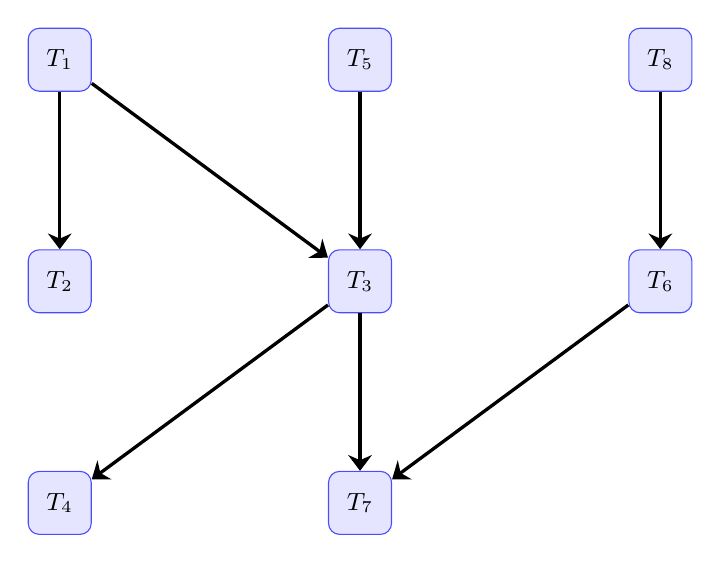
\begin{tikzpicture}[
        >={Stealth[length=2mm, width=3mm]},
        node distance=2cm and 3cm,
        auto
    ]

    % node placement
    \node[task] (T1) {$T_1$};
    \node[task, right=of T1] (T5) {$T_5$};
    \node[task, right=of T5] (T8) {$T_8$};

    \node[task, below=of T1] (T2) {$T_2$};
    \node[task, right=of T2] (T3) {$T_3$};
    \node[task, right=of T3] (T6) {$T_6$};

    \node[task, below=of T2] (T4) {$T_4$};
    \node[task, right=of T4] (T7) {$T_7$};

    % edges
    \draw[->, very thick] (T1) -- (T2);
    \draw[->, very thick] (T1) -- (T3);
    \draw[->, very thick] (T5) -- (T3);
    \draw[->, very thick] (T3) -- (T4);
    \draw[->, very thick] (T3) -- (T7);
    \draw[->, very thick] (T8) -- (T6);
    \draw[->, very thick] (T6) -- (T7);

    \end{tikzpicture}
    \caption{Task graph DAG where $T_i \to T_j$ indicates that task $T_j$ depends on the completion of task $T_i$.}\label{fig:task_dag}
\end{figure}

\subsection{Definitions}

Throught this paper, we will be using terms like \textit{successors}, \textit{predecessors} and \textit{lexicographically ordering}. The definitions for these terms are as follows.
\newline
Let $T_i$ and $T_j$ be tasks in the graph $G$.
\begin{itemize}
    \item \textbf{Predecessor}: If there is a path from $T_i$ to $T_j$, then $T_i$ is a \textbf{predecessor} of $T_j$.
    \item \textbf{Successor}: If there is a path from $T_i$ to $T_j$, then $T_j$ is a \textbf{successor} of $T_i$.
    \item \textbf{Immediate Predecessor}: If there is a direct edge $T_i \to T_j$, $T_i$ is an \textbf{immediate predecessor} of $T_j$.
    \item \textbf{Immediate Successor}: If there is a direct edge $T_i \to T_j$, $T_j$ is an \textbf{immediate successor} of $T_i$. The set of all immediate successors of a task $T$ is denoted $S(T)$.
\end{itemize}

\begin{definition}
    \textbf{Lexicographical ordering}: Let $A$ and $B$ be arrays of natural numbers.
    We say that $A$ is \textbf{less than} $B$ lexicographically, denoted $A <_{lex} B$, if there exists an index $i$ such that for all $j < i$, $A[j] = B[j]$ and $A[i] < B[i]$.
\end{definition}

\section{The \algname{}}

\subsection{How Does the Algorithm Work?}
Remember that the goal of the \algname{} is to find the optimal schedule $L^{*}$ for some task DAG $G$.
The \algname{} primarily employs a greedy approach, its core mechanism revolves around picking the \emph{least important} task in $G$ and scheduling it as late as possible in $L^{*}$.

\subsection{The Implementation}
Before we go into the full implementation, lets create a helper class to store our tasks and their dependencies.

\begin{lstlisting}[caption=TaskGraph class definition, label=lst:fib]
class TaskGraph:
    def __init__(self, tasks=None, successors=None):
        ...

    def number_of_tasks(self) -> int:
        ...

    def tasks(self):
        ...

    def add_task(self) -> int:
        ...

    def add_successor(self, predecessor, successor):
        ...

    def successors(self, v) -> list:
        ...
\end{lstlisting}

The successors are assume to be passed as a dictionary where the keys are task ids and the values are lists of task ids that depend on the key task.
Below I will use the class to store the task graph from figure~\ref{fig:task_dag}.

\begin{lstlisting}[caption=Creating TaskGraph from figure~\ref{fig:task_dag}, label=lst:taskgraph_example]
tasks = [i for i in range(1, 9)]
successors = {1: [2, 3], 3: [4, 7], 5: [3], 8: [6], 6: [7]}
G = TaskGraph(tasks, successors)
\end{lstlisting}

In the implementation we will also need a helper function to compare two lists lexicographically. I will be avoiding the implementation details, but the function is defined below.
\begin{lstlisting}[caption=Lexicographical comparison, label=lst:lex_compare]
def less_than_lexicographically(a: list, b: list) -> bool:
    ...
\end{lstlisting}

With these helper components defined, here is the full implementation of the \algname{}.

\begin{lstlisting}[caption=\algname{} implementation, label=lst:coffman_graham_algorithm]
def coffman_graham_algorithm(G: TaskGraph):
    r = G.number_of_tasks()
    k = 1
    alpha = {}

    for T in G.tasks():
        if not G.successors(T):
            alpha[T] = k
            k += 1

    while k <= r:
        N = {}
        for T in G.tasks():
            if T in alpha:
                continue

            all_successors_defined = True
            S_T = G.successors(T)

            for t in S_T:
                if t not in alpha:
                    all_successors_defined = False
                    break

            if all_successors_defined:
                N[T] = sorted([alpha[t] for t in S_T], reverse=True)

        current_min_n = None
        for n in N:
            if current_min_n == None:
                current_min_n = n
                continue

            lt_eq_lex = less_than_lexicographically(N[n], N[current_min_n])

            if lt_eq_lex:
                current_min_n = n
            elif N[n] == N[current_min_n]:
                if n < current_min_n:
                    current_min_n = n

        alpha[current_min_n] = k
        k += 1

    schedule = sorted(alpha.keys(), key=lambda task: alpha[task])
    return schedule[::-1]
\end{lstlisting}

\subsubsection{Example}
To illustrate the \algname{} working, consider the task graph from figure~\ref{fig:task_dag} represented in listing~\ref{lst:taskgraph_example}. 
We will run the \algname{} on this task graph to find the optimal schedule. See listing~\ref{lst:run_example} for the code to run the algorithm and the expected output.
\begin{lstlisting}[caption=Running \algname{} on example task graph, label=lst:run_example]
L = coffman_graham_algorithm(G)
print("Optimal Schedule: ", L)
> Optimal Schedule: [1, 5, 8, 3, 6, 7, 4, 2]
\end{lstlisting}

\subsection{Notes on the Implementation}
The presented implementation of the \algname{} has been analyzed with a worst-case time complexity of $O(n^3)$. 
It is important to note that, as stated in the paper~\cite{10.1007/BF00288685}, an optimal implementation can achieve a complexity of $O(n^2)$~\cite{10.1007/BF00288685}.
\section{Analysis and Correctness}

\subsection{Worst-Case Time Complexity}
The overall complexity is determined by the most time-consuming step:
\begin{itemize}
    \item \textbf{Main Loop $O(n)$:} The while loop runs from $k=1$ to $r$, where $r= \text{number of tasks in G}$. Therefore $n$ iterations where $n = \text{number of tasks in G}$.  
    \begin{itemize}
        \item
        \begin{lstlisting}[caption=Main Loop from listing~\ref{lst:coffman_graham_algorithm}, label=lst:coffman_graham_main_loop]
def coffman_graham_algorithm(G: TaskGraph):
    r = G.number_of_tasks()
    k = 1

    ...

    while k <= r:
        ...
        \end{lstlisting}
    \end{itemize}
    \item \textbf{Inner Loop $O(n)$:} The inner for loops goes over each job in $G$, potentially $n$ steps
    \begin{itemize}
        \item
        \begin{lstlisting}[caption=Inner for loop from listing~\ref{lst:coffman_graham_algorithm}, label=lst:coffman_graham_inner_loop]
def coffman_graham_algorithm(G: TaskGraph):
    ...

    while k <= r: # O(n) from previous step
        for T in G.tasks(): # O(n) this step
            ...
        \end{lstlisting}
    \end{itemize}
    \item \textbf{Inner Inner Loop $O(n)$:} The inner inner for loop goes over each job in $\mathbf{\text{S\_T}}$, potentially $n$ times    
    \begin{itemize}
        \item
        \begin{lstlisting}[caption=Inner Inner for loop from listing~\ref{lst:coffman_graham_algorithm}, label=lst:coffman_graham_inner_inner_loop]
def coffman_graham_algorithm(G: TaskGraph):
    ...

    while k <= r: # O(n) from first step
        for T in G.tasks(): # O(n) from previous step
            ...

            S_T = G.successors(T)

            for t in S_T: # O(n) this step
                ...
        \end{lstlisting}
        \item \textbf{What is $\mathbf{\text{S\_T}}$?:} $\mathbf{\text{S\_T}}$ is the array of immediate successors of some task. In the worst case, $|\mathbf{\text{S\_T}}| = \text{number of tasks in G} - 1$ which simplifies to $n - 1$. We remove the constant $-1$ for big O notation. Note that in practice, $|\mathbf{\text{S\_T}}|$ is often much smaller than $n$.
    \end{itemize}
\end{itemize}

Multiplying out these time complexities, we get that the total worst-case time complexity is
\[ O(n^3) \]

\subsection{Practical Run-Times}
For practical runtime testing, the \algname{} was ran on various datasets with increasing sizes. Each dataset size was ran through 5 times, with each time being randomized.

\begin{table}[h!]
    \centering
    \caption{Average Runtime of the Coffman-Graham Algorithm on Random DAGs.}\label{tab:coffman-graham-runtime}
    \begin{tabular}{|c|c|c|}
        \hline
        \textbf{Dataset Size ($N$)} & \textbf{Average Runtime (s)} & \textbf{Number of trials} \\
        \hline
        $10$ & $0.000039$ & $5$ \\
        \hline
        $50$ & $0.000770$ & $5$ \\
        \hline
        $100$ & $0.002070$ & $5$ \\
        \hline
        $500$ & $0.041140$ & $5$ \\
        \hline
        $1000$ & $0.162983$ & $5$ \\
        \hline
        $2000$ & $0.710861$ & $5$ \\
        \hline
    \end{tabular}
\end{table}

\textbf{Note:} The Dataset Size ($N$) in Table~\ref{tab:coffman-graham-runtime} refers to the number of tasks in the randomized DAG for each trial. In each randomized DAG, the dependencies were also generated randomly.

\subsection{Correctness}
The correctness of the \algname{} is proven in the original paper~\cite{10.1007/BF00288685}.
In short, the proof shows that for any task graph $G$ you can create a group of tasks, such that every task in the group has to be completed before the next group of tasks can be started.
The proof then shows that for each of these groups, you require at least $n_k$ timesteps to complete all tasks in group $k$ where $n_k$ is the number of tasks in group $k$.
Finally, the proof shows the sum of all these $n_k$'s is equal to the makespan of the schedule $L^{*}$ produced by the \algname{}.

\section{Extensions into $3$ or more processors}
A natural question that arises is whether the \algname{} can be extended to handle more than two processors. If $m$ is the number of processors, then for all fixed $m >= 3$ finding the optimal schedule of a task graph on $m$ processors is an \textbf{open problem}~\cite{10.5555/574848}.
However it was shown that if the number of processors $m$ is part of the input, then finding the optimal schedule is NP-complete~\cite{10.5555/574848}.

\section{Conclusion}
The \algname{} is an efficient algorithm for finding the optimal schedule of a task graph given two processors. Our implementation achieves a worst-case time complexity of $O(n^3)$.

\printbibliography{}

\end{document}
